\documentclass[border=1pt]{standalone}
\usepackage[dvipsnames]{xcolor}
\usepackage{tikz}                       % Graphen und kommutative Diagramme
\usetikzlibrary{patterns}               % Um schraffierte Formen in der tikzpicture-Umgebung zu zeichnen.
\newcommand{\ul}[1]{\underline{\smash{#1}}}

\begin{document}
\centering
\begin{minipage}{.8\textwidth}
\centering
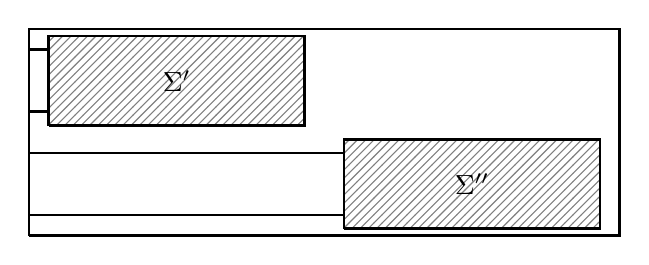
\begin{tikzpicture}[yscale=.7, xscale=1, x=1.25cm, y=1.25cm, line width=1pt]
    \draw (0,0) -- (6,0) -- (6,3) -- (0,3) -- (0,0);
    
    \filldraw[pattern=north east lines, pattern color=black!50] (0.2, 1.6) -- (2.8, 1.6) -- (2.8, 2.9) -- (0.2, 2.9) -- (0.2, 1.6);
    \filldraw[pattern=north east lines, pattern color=black!50] (3.2, 0.1) -- (5.8, 0.1) -- (5.8, 1.4) -- (3.2, 1.4) -- (3.2, 0.1);
    
    \draw (0, 1.8) -- (0.2, 1.8);
    \draw (0, 2.7) -- (0.2, 2.7);
    
    \draw (0, 0.3) -- (3.2, 0.3);
    \draw (0, 1.2) -- (3.2, 1.2); 
    
    \node at (1.5, 2.25) {$\Sigma'$};
    \node at (4.5, 0.75) {$\Sigma''$};
\end{tikzpicture}
\end{minipage}
\end{document}
